
\subsection{Simulation Study Results}

In this section, we present the substantial interaction effects on RPB and RMSE results for interactions between pairs of conditions. The full simulation results are available in the supplementary materials. 

\subsubsection{Convergence}

REML paired with all the variance formulae (except Fisher TF) had occasional issues converging across conditions. We ran 1,500 replications of each condition to ensure that we captured results from analysis of at least 1,000 converged replications permethod. Across all 1,500 replications, all of the non-convergence for REML occurred in the small number of clusters condition ($\mathcal{U}$[30, 50]). The lowest convergence rate was 99.27\% across conditions. In order to compare the same number of replication datasets for each condition, the graphs only summarize the same set of 1,000 replications per condition.

\subsubsection{Pooled ICC estimate}

Below are the results for the RPB of the pooled ICC estimate (Figures: \ref{fig:RPBk}:\ref{fig:RMSEtau}). Figure \ref{fig:RPBk} presents the RPB estimates as a function of number of estimates being pooled ($k$) and the true generating ICC values ($\rho$). As can be seen from the graph, we found no differences between using REML and RVE when pooling ICC estimates across the conditions we evaluated. Furthermore, we found no differences as a function of the number of ICC estimates pooled using 20, 50, or 100 estimates. However, using the Fisher formula for $v_r$ that uses a normalizing transformation of $\rho$ (Fisher TF; Equation  \ref{fisher_transformed_ICC}) performs best across the different $v_r$ formulae when used as the inverse weight formula. h larger $\rho$, $0.25$,  the $v_r$ formulae did not matter, and all formulae resulted in unbiased estimates. 
\begin{figure*}[h!]
\centerline{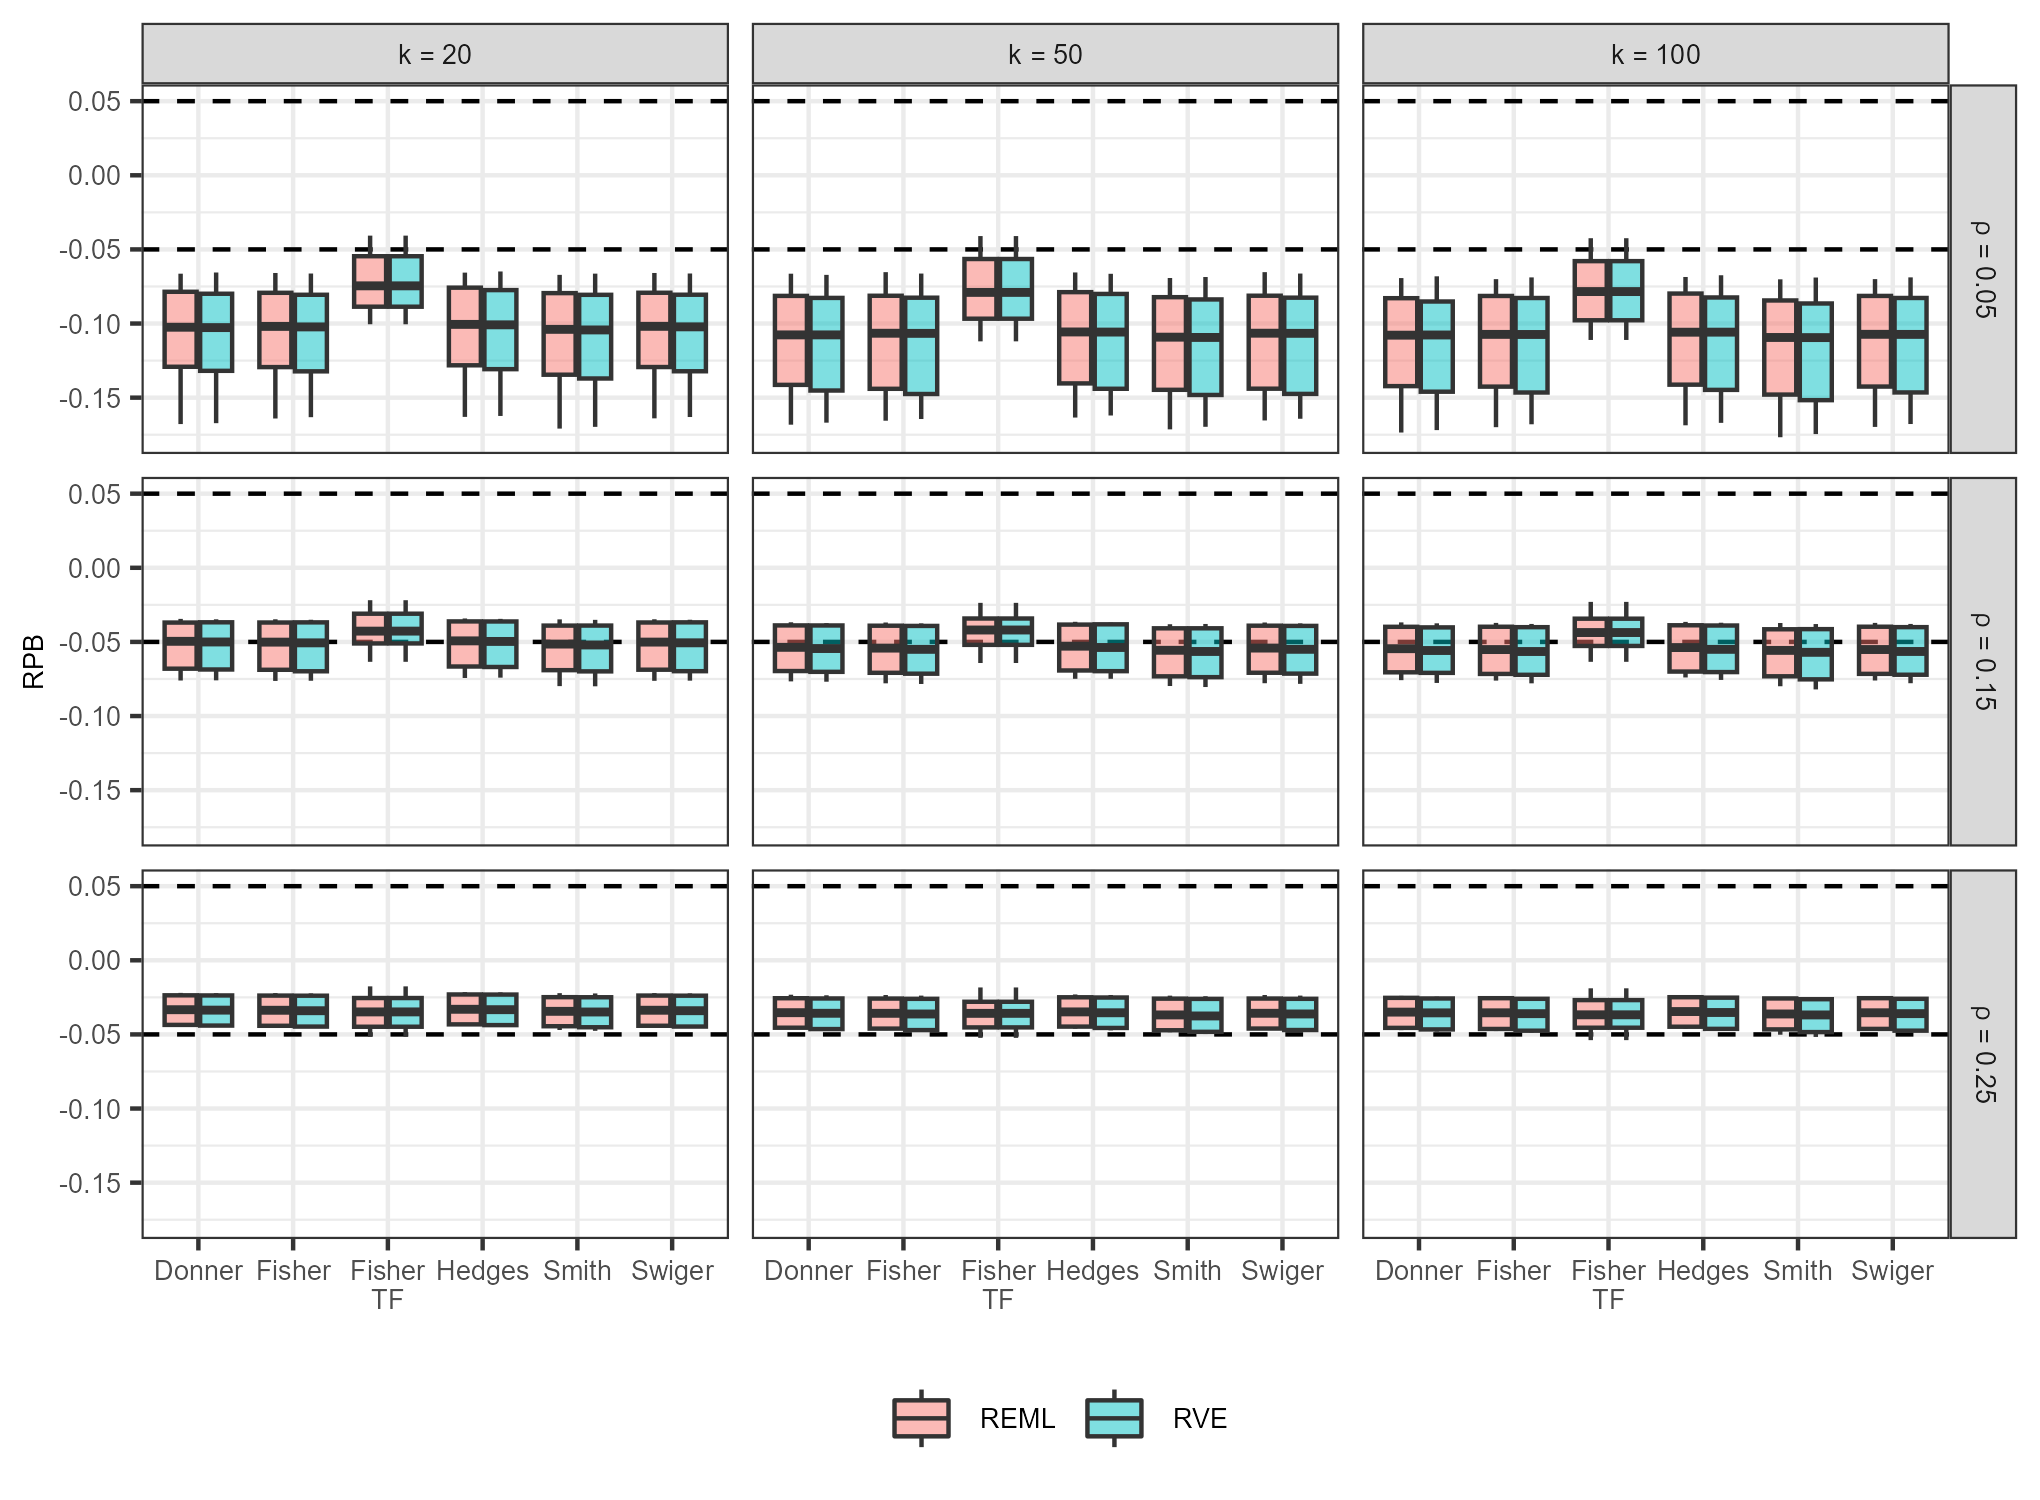
\includegraphics{Main/RPB_numICC.png}}
    \caption{The RPB of the pooled ICC estimates by the method of pooling, number of ICC estimates pooled ($k$) and the generating true ICC ($\rho$). \label{fig:RPBk}}
\end{figure*}

Figure \ref{fig:RPBtau} displays the RPB estimates as a function of between-study heterogeneity ($\tau$) and the true generating ICC values ($\rho$). There were very small differences in the degree of between-study heterogeneity that we evaluated. Higher between-study heterogeneity when the true generating ICC values are small ($\rho = .05$)resulted in negatively biased estimates across all methods with the Fisher TF variance formula resulting in the least biased estimates. For the $\rho$ values of 0.15, the estimates were very close to lacking substantial bias and no substantial bias was found when $\rho$ was generated using a value of 0.25. All the variance formulae underestimated the overall pooled effect. 
\begin{figure*}[h!]
\centerline{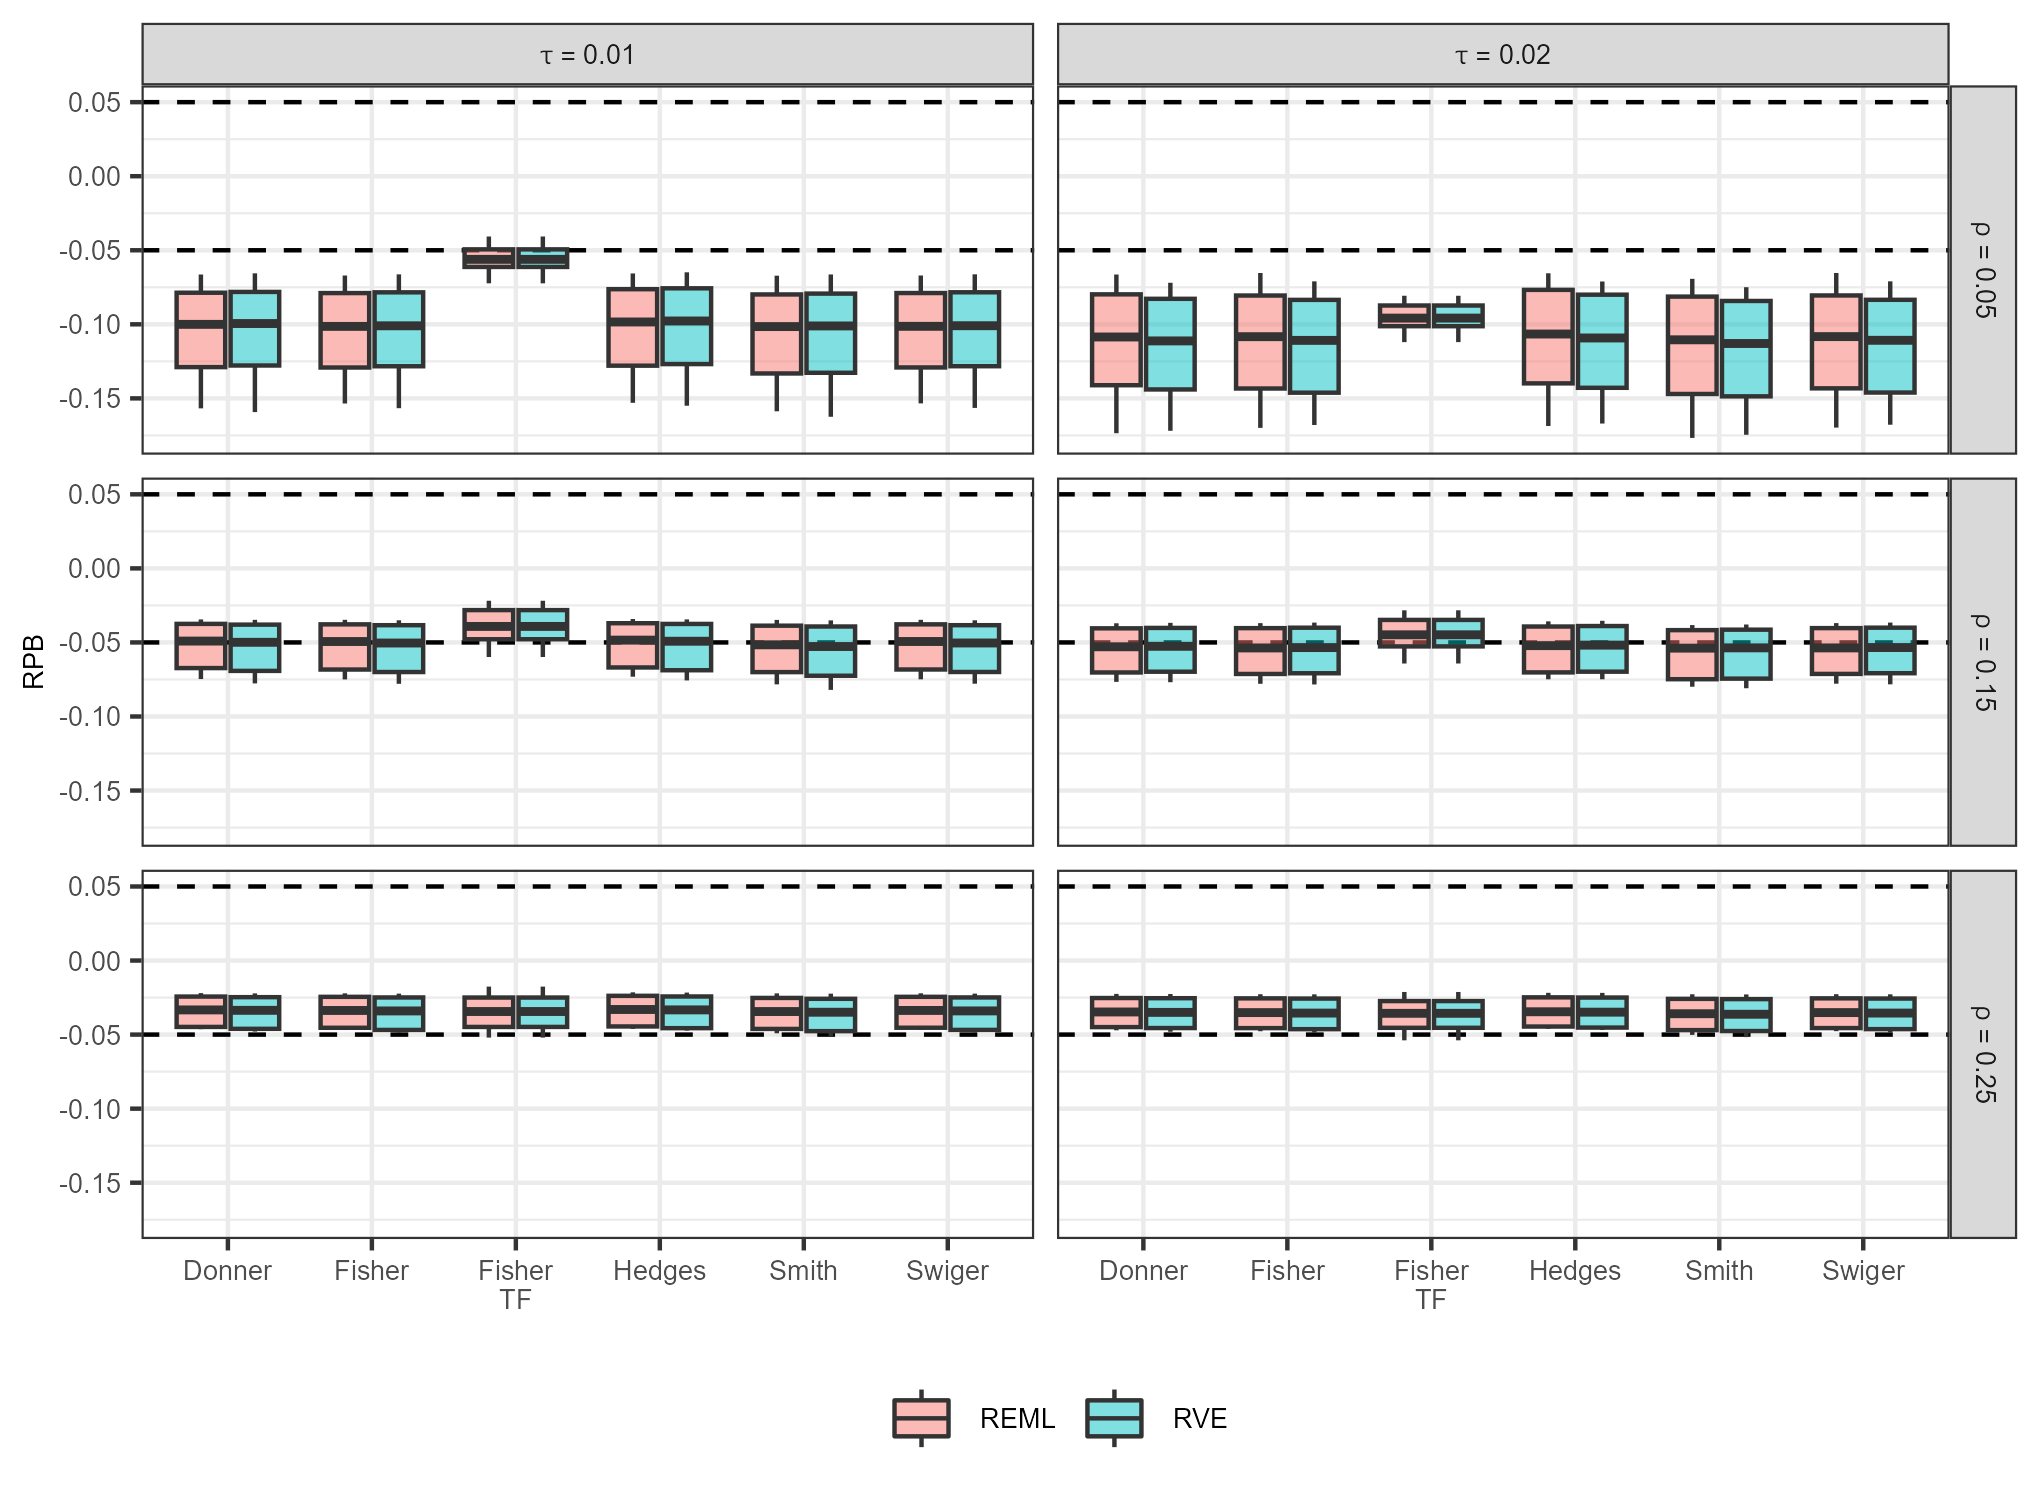
\includegraphics{Main/RPB_tau.png}}
\caption{The RPB of the pooled ICC estimates by the method of pooling, between study heterogeneity ($\tau$) and the generating true ICC ($\rho$). \label{fig:RPBtau}}
\end{figure*}

Figure \ref{fig:RMSEk} provides the results for the RMSE of the pooled ICC estimate as a function of number of estimates being pooled ($k$) and the true generating ICC values ($\rho$). Consistent with the RPB results, the Fisher TF variance formula results in the lowest RMSE for small true generating ICC values ($\rho=0.05$ and $\rho=0.15$).
\begin{figure*}[h!]
\centerline{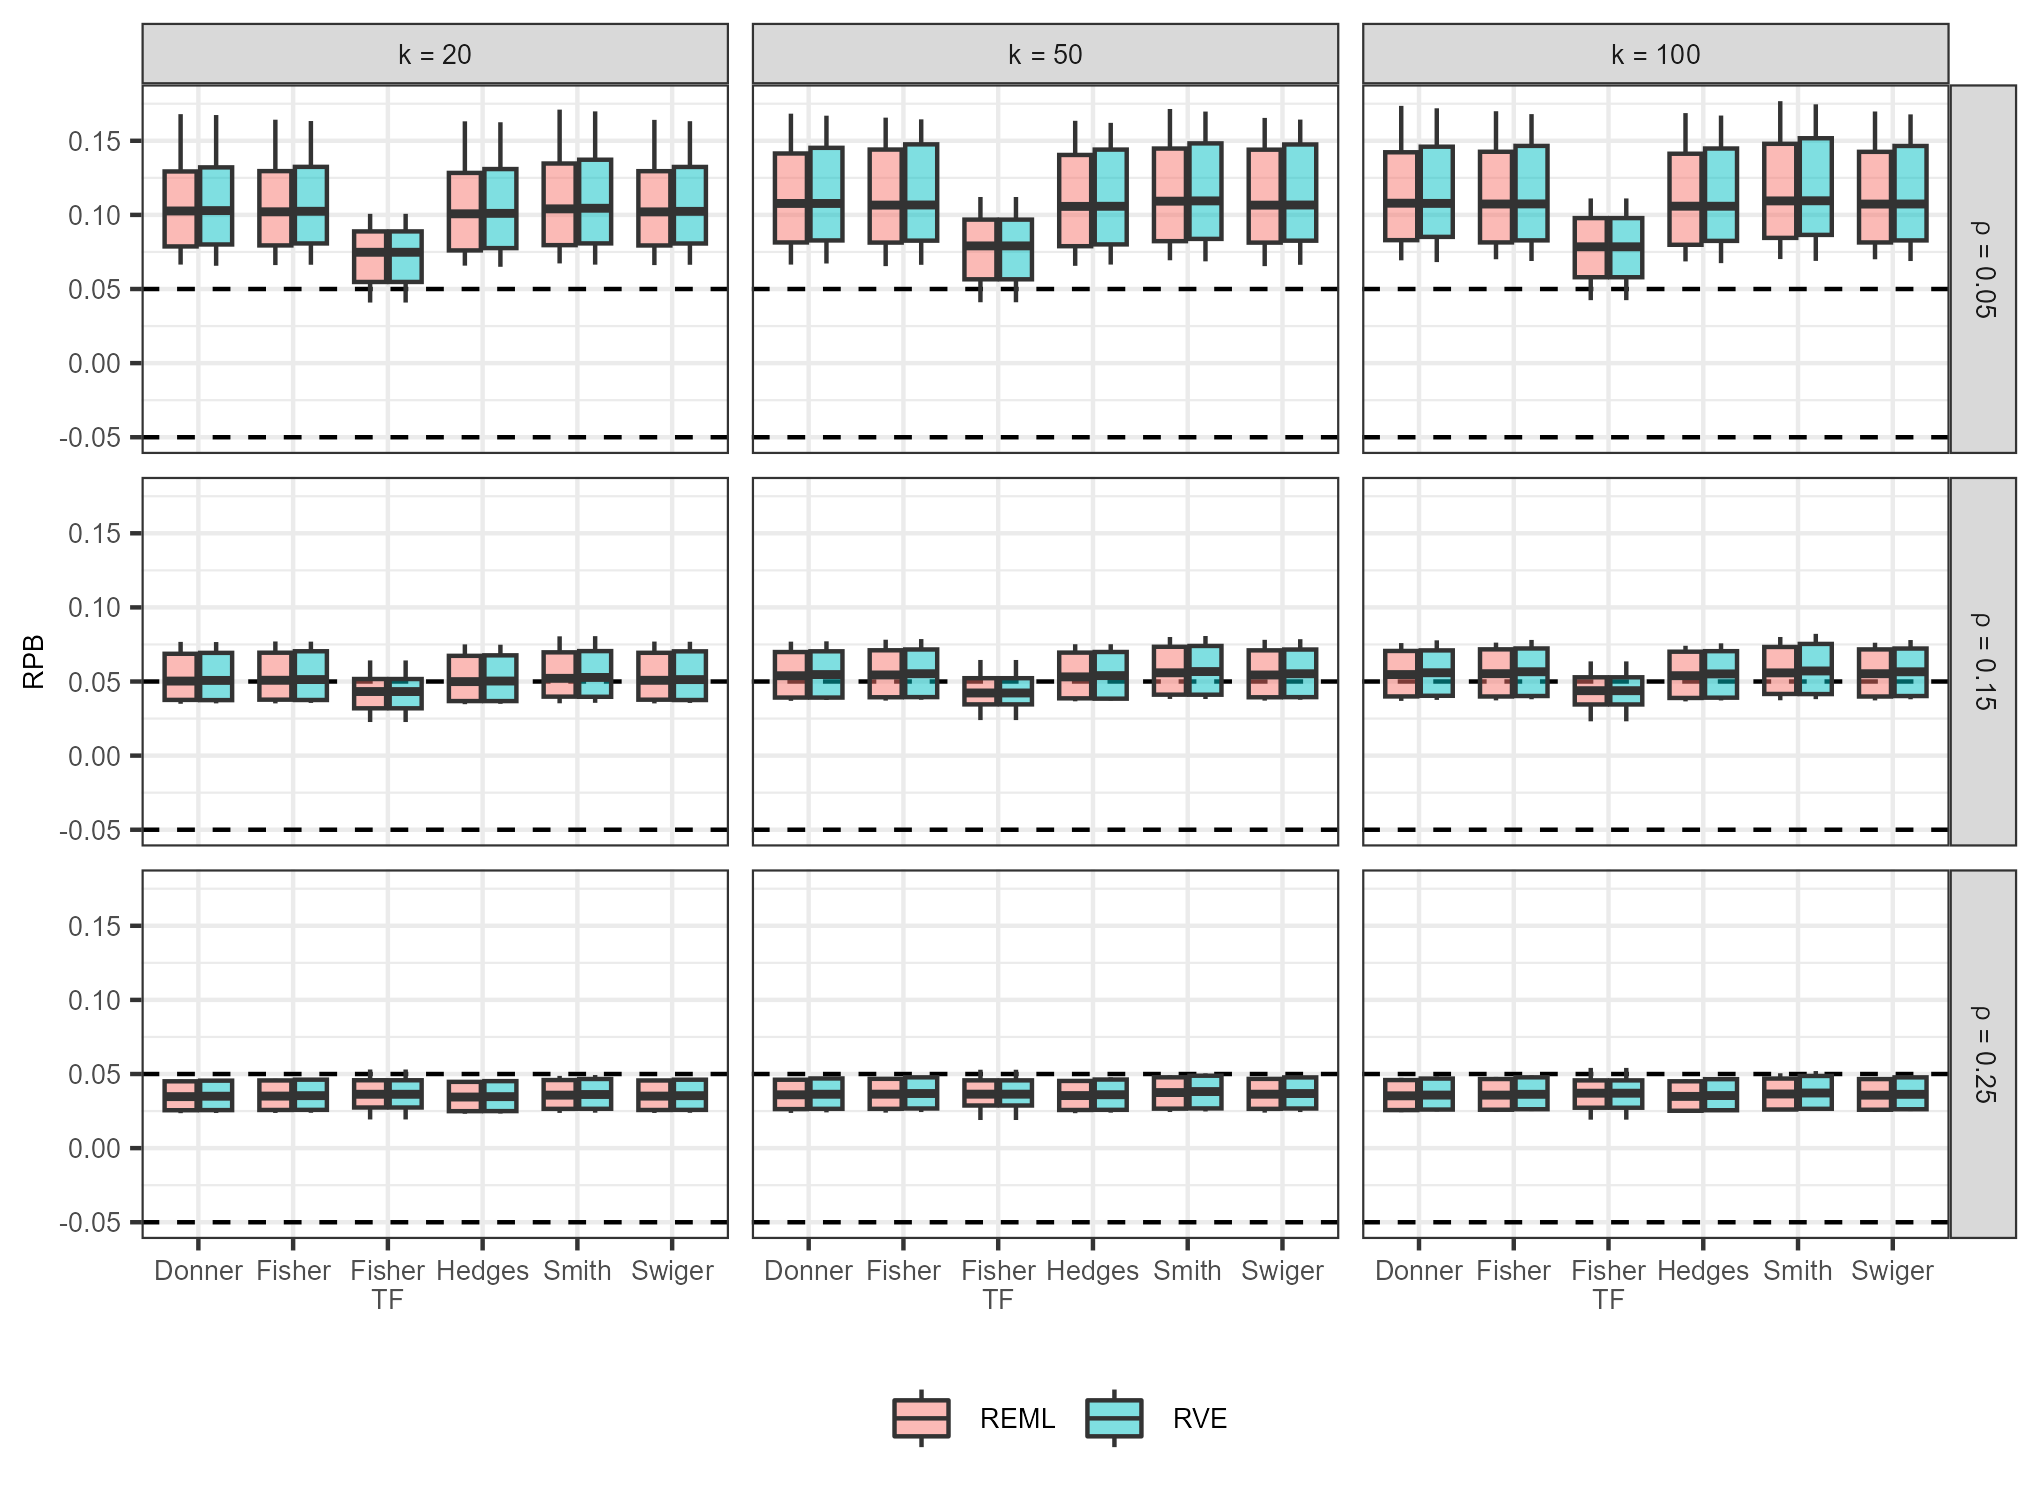
\includegraphics{Main/RMSE_numICC.png}}
    \caption{The RMSE using of the pooled ICC estimates by the method of pooling, number of ICC estimates pooled ($k$) and the generating true ICC ($\rho$).\label{fig:RMSEk} }
\end{figure*}


Figure \ref{fig:RMSEtau} contains the results for the RMSE of the pooled ICC estimate as a function of between-study heterogeneity ($\tau$) and the true generating ICC values ($\rho$). 

\begin{figure*}[h!]
\centerline{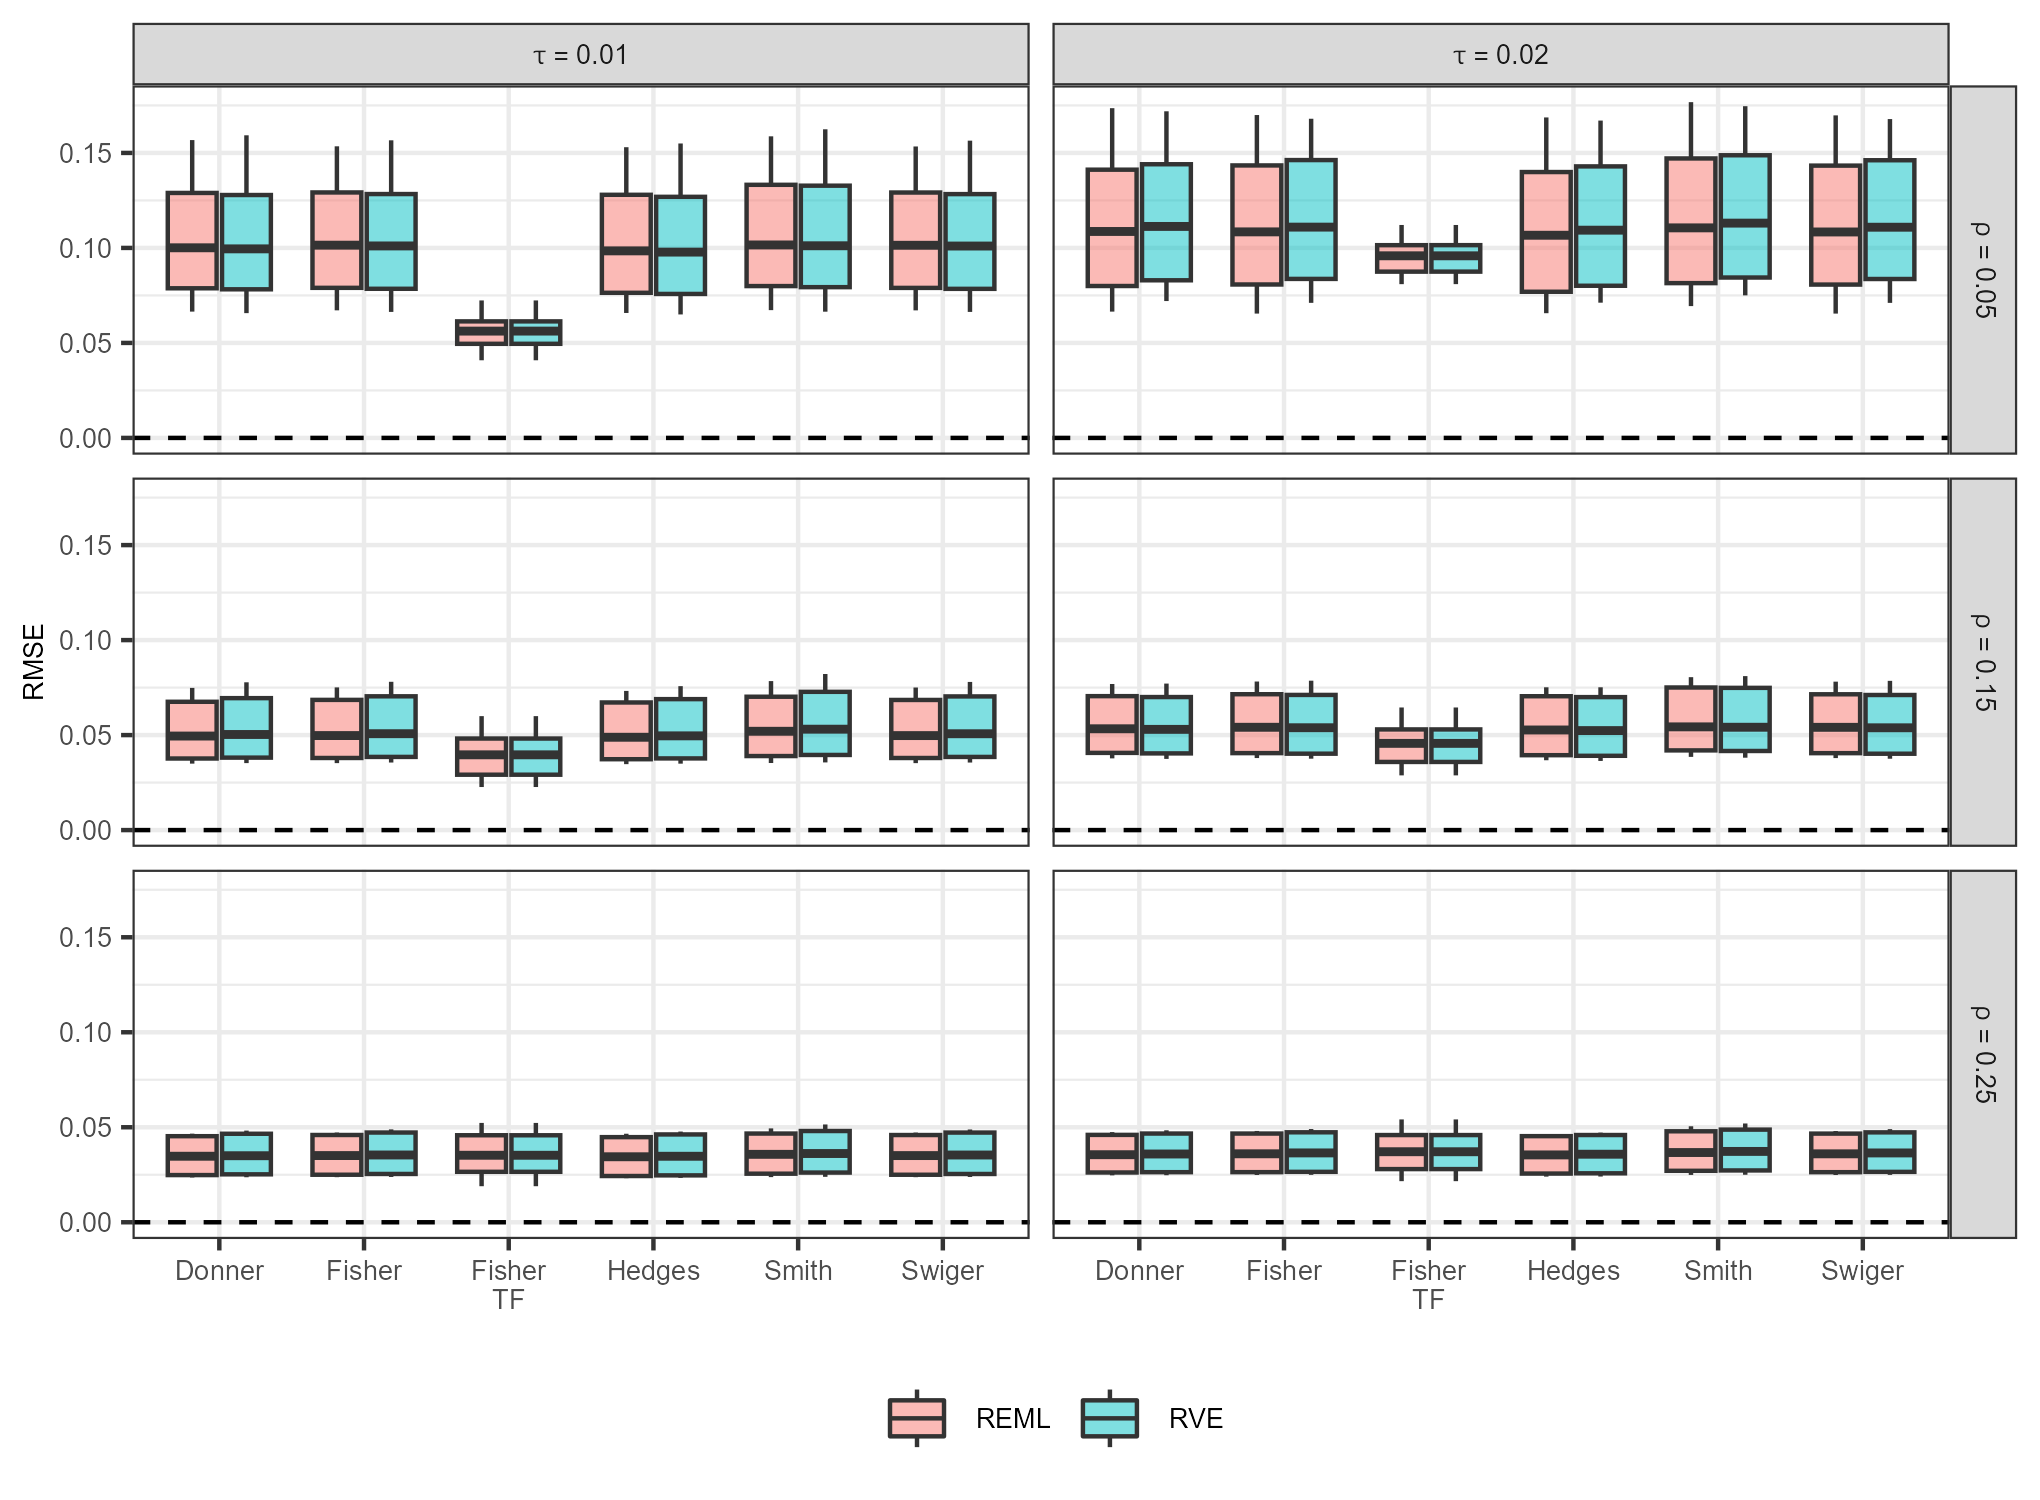
\includegraphics{Main/RMSE_tau.png}}
    \caption{The RMSE of the pooled ICC estimates by the method of pooling, between study heterogeneity ($\tau$) and the generating true ICC ($\rho$). \label{fig:RMSEtau} }
\end{figure*}


%%%%%%%%%%%%%%%%%%%%%%%%%%%%%%%%%%%%%%%

\subsubsection{SE of the Pooled ICC Estimate}




Figure \ref{fig:RPBkse_k} displays results for the RSEB of the pooled ICC estimate as a function of number of estimates being pooled ($k$) and the true generating ICC values ($\rho$). In addition, the number of ICC estimates pooled does not make a difference in RSEB across the conditions we evaluated. These results were consistent with other conditions we evaluated  (results in Supplementary Materials). 



\begin{figure*}[h!]
\centerline{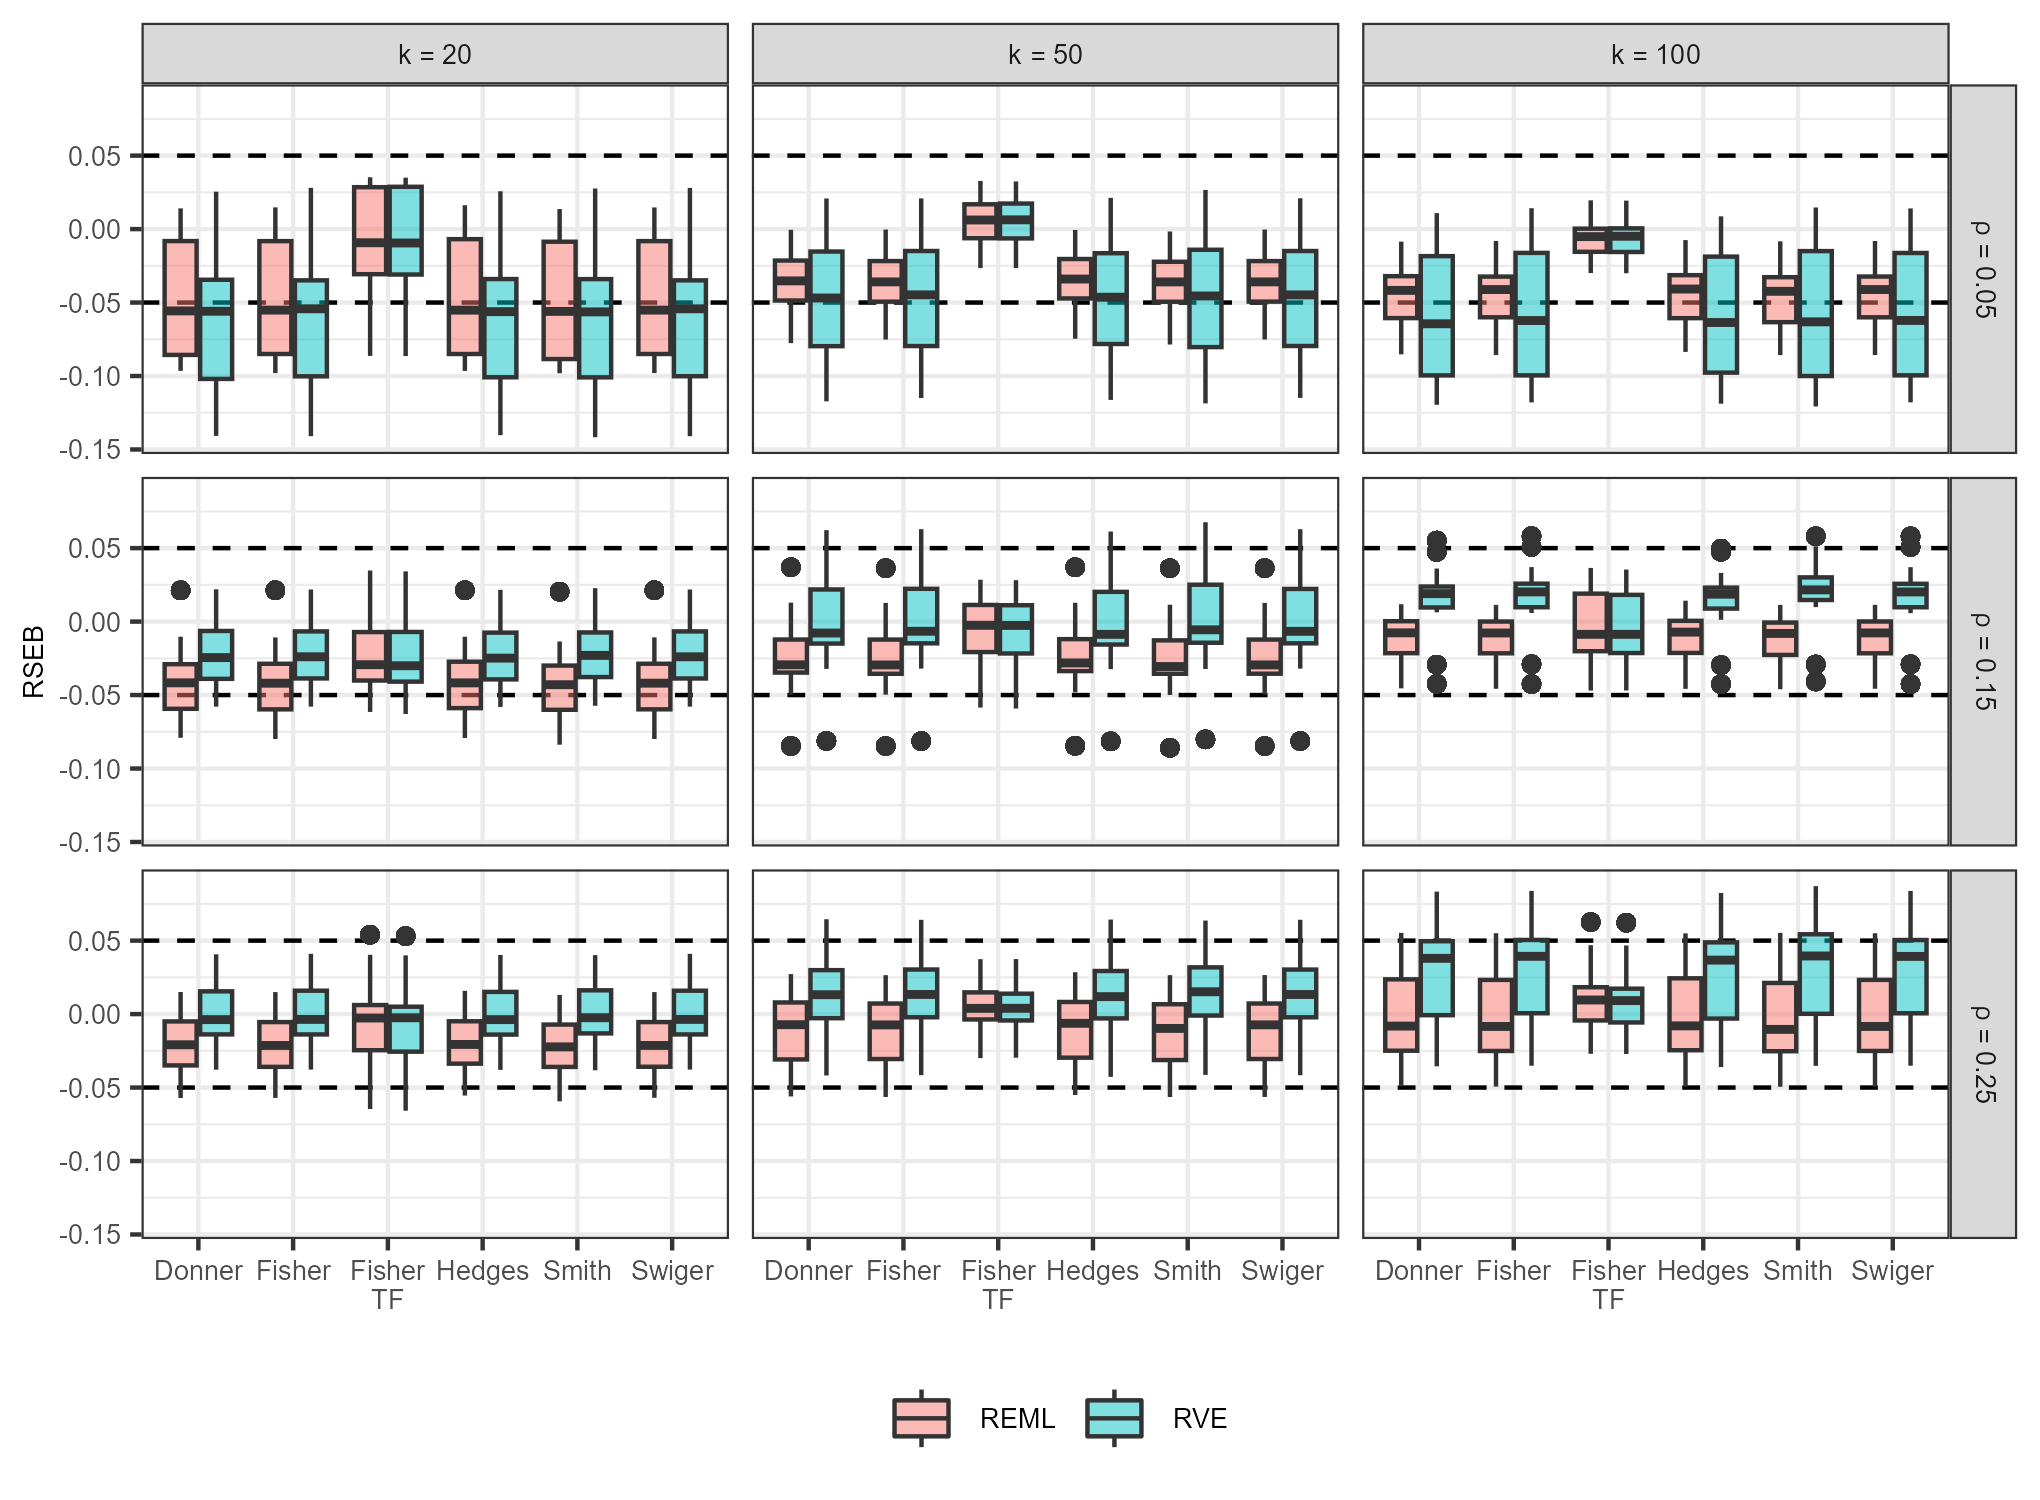
\includegraphics{Main/RSE_numICC.png}}
    \caption{The RSEB of the pooled ICC estimates by the method of pooling, number of ICC estimates pooled ($k$) and the generating true ICC ($\rho$). \label{fig:RPBkse_k}}
\end{figure*}




%%%%%%%%%%%%%%%%%%%%%%%%%%%%%%%%%%%%%%%%%%%%


\subsubsection{ Level 2 Variance of Primary Studies}


\paragraph{Relative parameter bias}

The Figures below display results for the RPB of the L2 variance. Figure \ref{fig:RPB_L2_tau} below provides a box plot of level-2 variances estimates by between-study heterogeneity. As can be seen in the Figure, for $\tau = 0.02$ and $\rho = 0.05$, the level-2 variance estimates were slightly biased when the generating true ICC was small ($\rho = 0.05$). We also wanted to confirm that the level-2 variance of the primary study was recovered well across the number of clusters condition. As can be seen in Figure \ref{fig:RPB_L2_j_mean} when we drew the number of clusters from a $U(30, 50)$ and when $\rho = 0.05$ this resulted in slightly biased estimates of the level-2 variance. Otherwise, across conditions, estimation of the level-2 variance was not substantially biased.

\begin{figure*}[h!]
\centerline{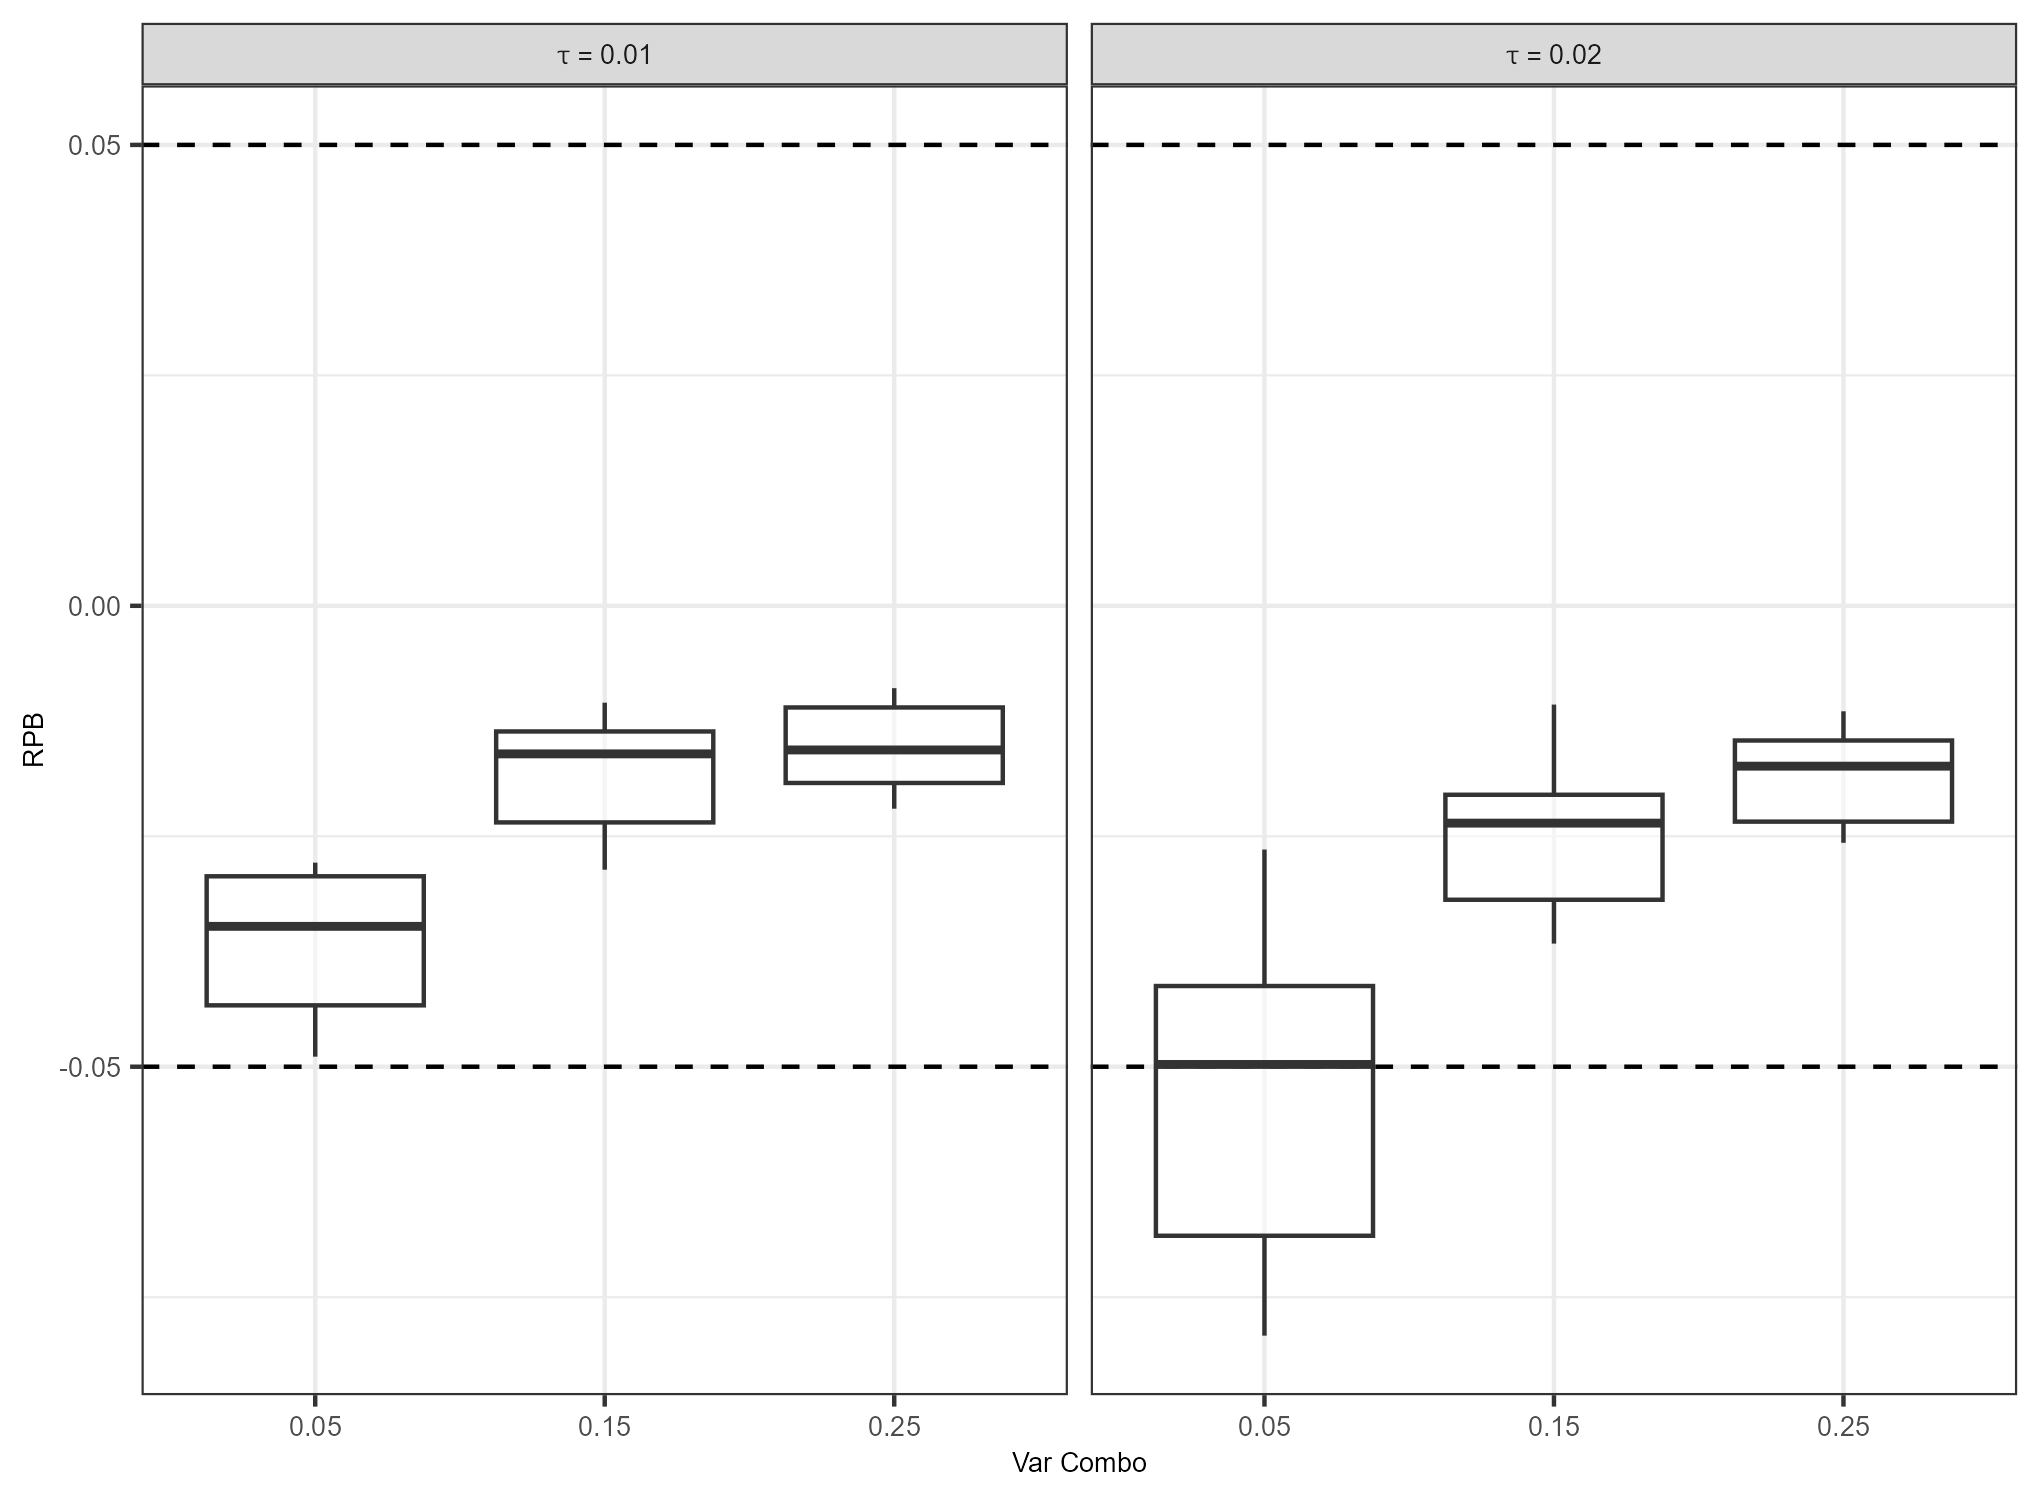
\includegraphics{Main/RPB_L2_tau_mean.png}}
    \caption{The RPB of the level-2 variance estimate by between study heterogeneity ($\tau$).\label{fig:RPB_L2_tau}}
\end{figure*}



\begin{figure}[h!]
\centerline{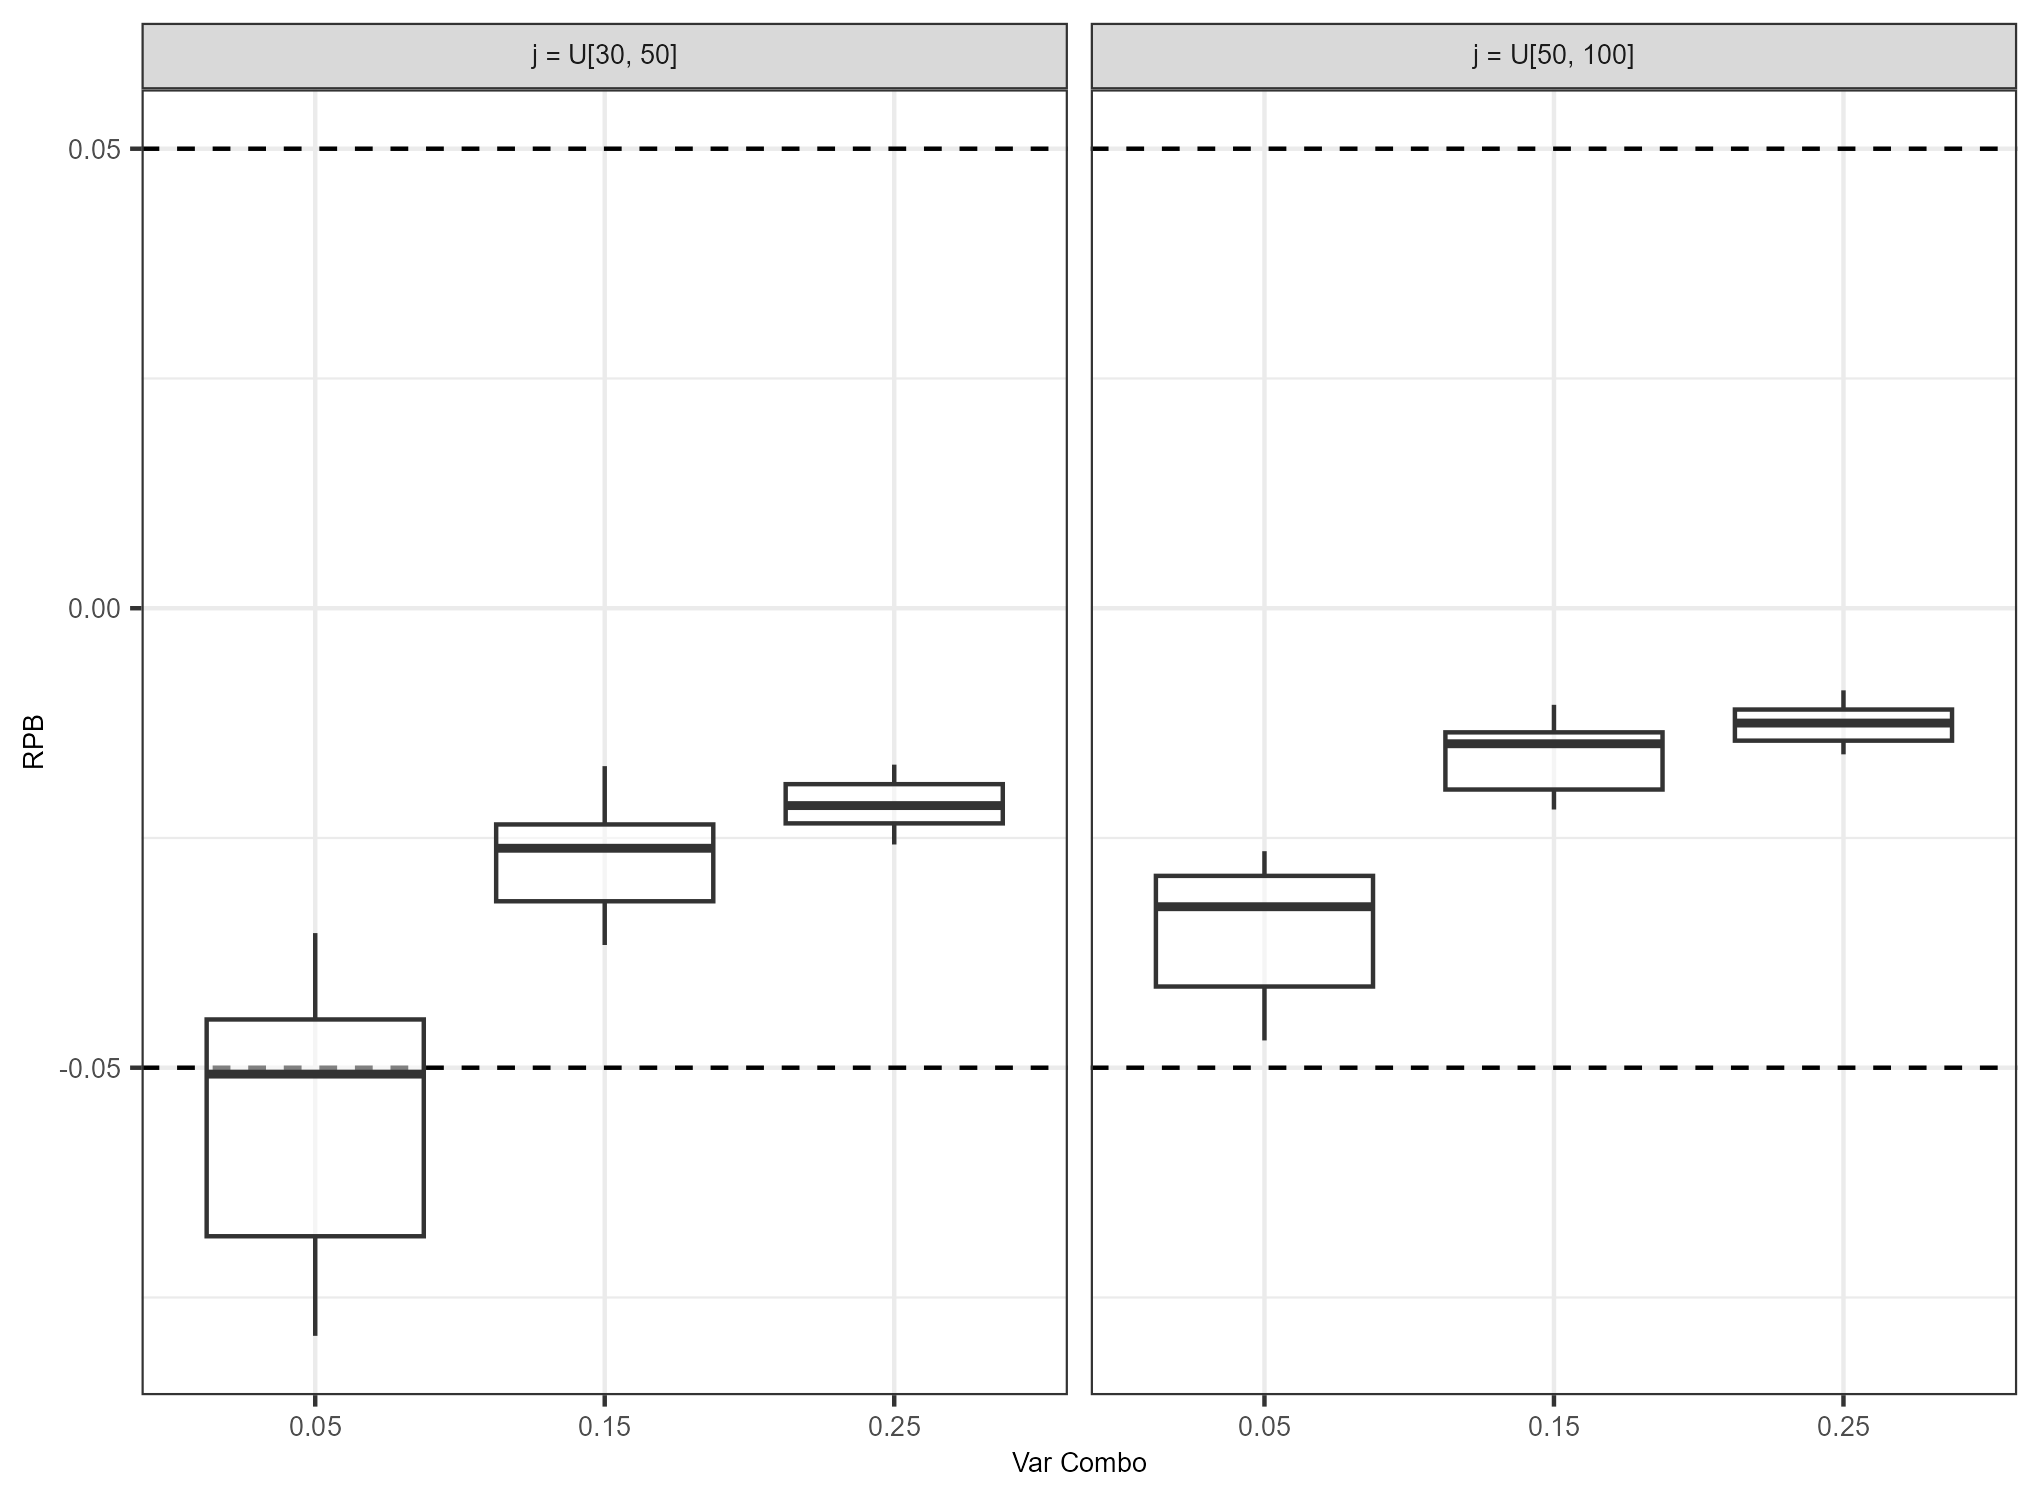
\includegraphics{Main/RPB_L2_j_mean.png}}
    \caption{The RPB of the level-2 variance estimate by number of clusters ($\tau$).\label{fig:RPB_L2_j_mean}}
\end{figure}

